\section{CMOS-Logik}

\begin{itemize}
    \item Entweder leitender Pfad nach $V_{SS}$ (NMOS) oder $V_{DD}$ (PMOS)
    \item Kein statischer Stromverbrauch
    \item Langsamer als Bipolar
    \item Symmetrische Schaltschwellen
    \item Höhere Speisespannung \textrightarrow weniger propagation delay
\end{itemize}


\subsection{Grundgatter in CMOS-Logik}

\begin{minipage}[t]{0.32\columnwidth}
    \begin{center}
        \textbf{Inverter} \\
    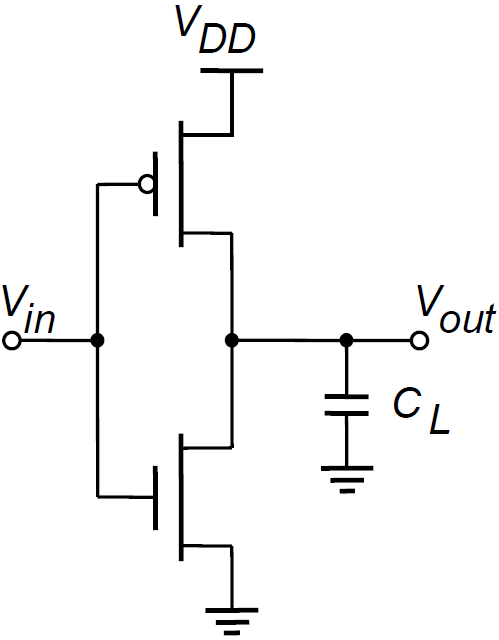
\includegraphics[width=\columnwidth]{images/cmos_inverter.png}
    \end{center}
\end{minipage}
\hfill
\begin{minipage}[t]{0.27\columnwidth}
    \begin{center}
        \textbf{NAND-Gate} \\
    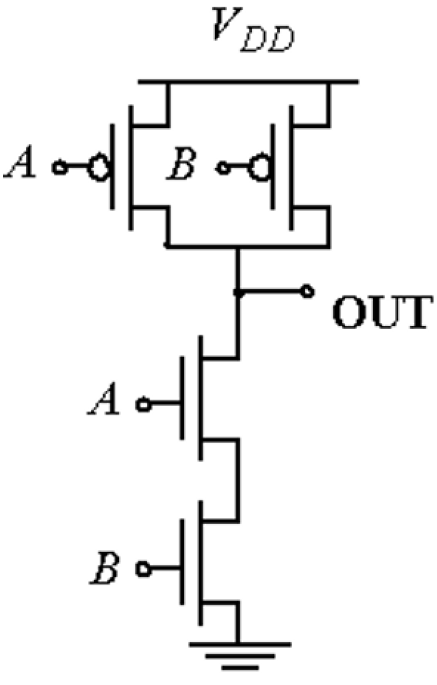
\includegraphics[width=\columnwidth]{images/cmos_nand_2.png}
    \end{center}
\end{minipage}
\hfill
\begin{minipage}[t]{0.38\columnwidth}
    \begin{center}
        \textbf{NOR-Gate} \\
    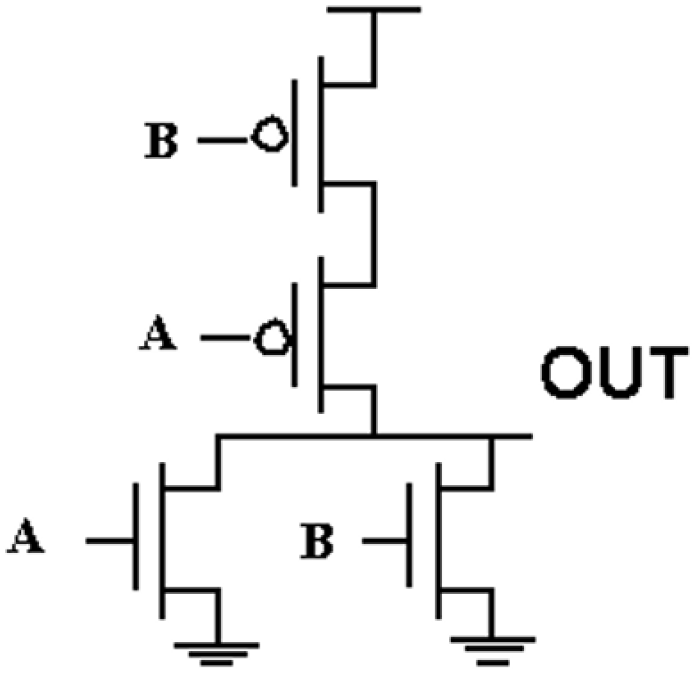
\includegraphics[width=\columnwidth]{images/cmos_nor.png}
    \end{center}
\end{minipage}


\subsection{Dualität NMOS - PMOS}